\documentclass[11pt]{article}
\usepackage[utf8]{inputenc}
\usepackage[T1]{fontenc}
\usepackage[spanish,es-nodecimaldot]{babel}
\usepackage{amsmath,amssymb,booktabs,geometry,graphicx,hyperref,microtype,xcolor}
\geometry{margin=2.4cm}
\hypersetup{colorlinks=true,linkcolor=blue!50!black,urlcolor=blue!60!black,citecolor=blue!50!black}
\title{Forecasting probabilístico como capa de salida para RiskGate\\\large Experimento preliminar con GJR--GARCH y DeepAR-style}
\author{RiskGate Research}
\date{20 de julio de 2026}

\begin{document}
\maketitle

\begin{abstract}
Se estudia si un pronóstico probabilístico diario puede mejorar una regla de salida para posiciones largas.
Se comparan buy-and-hold, un filtro EWMA, GJR--GARCH(1,1) con innovaciones $t$ y una red recurrente global
tipo DeepAR. Los umbrales se seleccionan exclusivamente en 2022--2023 y se evalúan desde 2024 sobre diez
activos líquidos, con costo de 5 puntos base por cambio de exposición. GJR--GARCH elevó el Sharpe de 1.16 a
1.31 y redujo el drawdown máximo de $-27.5\%$ a $-18.5\%$, sacrificando retorno. Sin embargo, el intervalo
bootstrap al 90\% de la diferencia de Sharpe incluye cero. DeepAR-style quedó mal calibrado y no mostró valor.
La evidencia justifica continuar investigando una capa de control de volatilidad, pero no integrar todavía una
recomendación automática de venta en RiskGate.
\end{abstract}

\section{Pregunta de investigación}
La pregunta no es si un modelo puede predecir el precio puntual, sino si su distribución predictiva mejora una
decisión accionable: mantener o reducir una posición durante la siguiente sesión. Las hipótesis registradas son:
\begin{enumerate}
  \item un filtro de volatilidad GJR--GARCH puede reducir drawdown y mejorar rendimiento ajustado por riesgo;
  \item un modelo recurrente probabilístico puede aportar señal direccional adicional;
  \item cualquier modelo complejo debe superar a EWMA, no sólo a buy-and-hold.
\end{enumerate}
Esta es una prueba sobre retornos del subyacente. No valida aún el momento óptimo de cierre de una opción,
porque no se dispone de series históricas completas de bid/ask, volatilidad implícita y griegas.

\section{Teoría}
\subsection{GJR--GARCH--$t$}
Sea $r_t=\mu+\epsilon_t$, con $\epsilon_t=\sigma_t z_t$ y $z_t$ estandarizado con distribución $t$.
El modelo asimétrico utilizado es
\begin{equation}
 \sigma_t^2=\omega+\alpha\epsilon_{t-1}^2+
 \gamma\epsilon_{t-1}^2\mathbf{1}\{\epsilon_{t-1}<0\}+\beta\sigma_{t-1}^2.
\end{equation}
El parámetro $\gamma$ captura que choques negativos pueden elevar más la volatilidad. El modelo pronostica
riesgo condicional, no dirección. Por ello la regla sale del mercado cuando $\hat\sigma_{t+1}$ rebasa un umbral
seleccionado fuera del conjunto de prueba. Como documenta el estudio de PF-Learning que motivó este trabajo,
GJR--GARCH puede funcionar en regímenes cercanos a volatilidad estocástica clásica y fallar ante saltos
acoplados al estado; se trata, entonces, de un filtro y no de una autoridad de venta.

\subsection{DeepAR-style}
DeepAR modela una familia de series mediante una red autorregresiva global y emite los parámetros de una
distribución condicional \cite{deepar}. En esta primera implementación, un LSTM de dos capas recibe una ventana
de 40 sesiones con retorno, retorno absoluto, volatilidades a 5 y 20 días, momentum y cambio de volumen. La
cabeza gaussiana produce $(\mu_t,\sigma_t)$ y se minimiza
\begin{equation}
 \mathcal L_t=\log\sigma_t+\frac{1}{2}\left(\frac{r_{t+1}-\mu_t}{\sigma_t}\right)^2.
\end{equation}
La regla mantiene exposición cuando $P(r_{t+1}<0)$ no supera el umbral validado. Se denomina
\emph{DeepAR-style}, no DeepAR canónico: esta versión usa emisión gaussiana, covariables limitadas y un solo
entrenamiento global.

\subsection{De forecast a decisión}
Para cada activo, la rentabilidad de la capa de salida es
\begin{equation}
 r^{\mathrm{strat}}_{t+1}=a_t r_{t+1}-c|a_t-a_{t-1}|,\qquad a_t\in\{0,1\},
\end{equation}
donde $a_t$ se conoce al cierre de $t$ y $c=5$ puntos base. Esta alineación evita utilizar el retorno futuro para
decidir. Una recomendación posterior para opciones deberá comparar la utilidad de mantener contra cerrar,
traduciendo la distribución del subyacente a P\&L mediante el payoff y las griegas.

\section{Diseño experimental}
Se descargaron precios diarios ajustados desde el endpoint público de Yahoo Finance para SPY, QQQ, IWM,
AAPL, MSFT, NVDA, AMZN, GOOGL, META y TSLA. La división cronológica quedó fijada así:
\begin{itemize}
  \item entrenamiento: 2015--2021;
  \item validación y selección de umbrales: 2022--2023;
  \item prueba final: 1 de enero de 2024 hasta la última observación disponible al ejecutar el estudio.
\end{itemize}
El conjunto de prueba contiene 6,370 observaciones activo--día. Los umbrales candidatos se fijaron antes de
examinar el test: probabilidades entre 0.50 y 0.75 para DeepAR-style y cuantiles 65--95 de volatilidad para
EWMA/GARCH. Se eligió el mayor Sharpe en validación. Las métricas son retorno y volatilidad anualizados,
Sharpe sin tasa libre de riesgo, drawdown máximo, riqueza final, exposición y rotación.

La incertidumbre se estima con 2,000 réplicas de bootstrap de bloques móviles de 20 sesiones. Este bootstrap
respeta parcialmente la dependencia temporal, aunque no corrige selección entre múltiples especificaciones.

\section{Resultados}
\begin{table}[ht]
\centering
\caption{Resultados fuera de muestra desde 2024.}
\begin{tabular}{lrrrrrr}
\toprule
Modelo & Ret. anual & Vol. anual & Sharpe & Max DD & Exposición & Cambios \\
\midrule
Buy \& hold   & 27.1\% & 23.2\% & 1.16 & $-27.5\%$ & 100.0\% & 0 \\
EWMA          & 16.3\% & 14.5\% & 1.13 & $-16.8\%$ & 77.0\% & 163 \\
GJR--GARCH--$t$ & 20.3\% & 15.5\% & 1.31 & $-18.5\%$ & 77.0\% & 36 \\
DeepAR-style  & 1.2\%  & 1.9\%  & 0.64 & $-2.8\%$  & 0.5\%  & 44 \\
\bottomrule
\end{tabular}
\end{table}

\begin{figure}[ht]
\centering
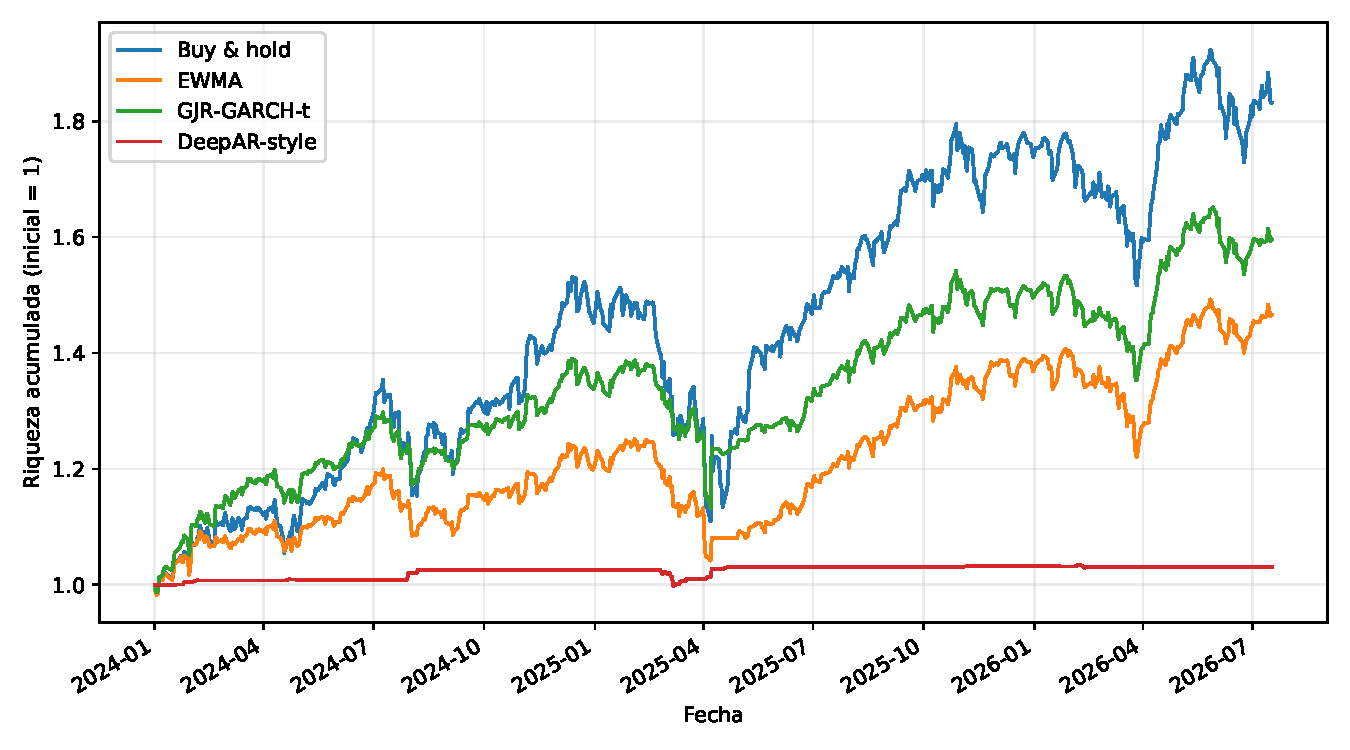
\includegraphics[width=.9\textwidth]{results/equity_curves.pdf}
\caption{Riqueza acumulada neta del costo supuesto, inicializada en uno.}
\end{figure}

GJR--GARCH produjo la mejor razón retorno/riesgo y mucha menos rotación que EWMA. No obstante, la mediana
bootstrap de la mejora de Sharpe sobre buy-and-hold fue 0.07, con intervalo al 90\% de $[-0.43,0.51]$.
La diferencia media de retorno diario tuvo intervalo $[-6.65,1.63]$ puntos base. En consecuencia, no se puede
descartar que la mejora observada sea ruido. Además, el umbral global dejó a TSLA sin exposición y generó
exposiciones muy diferentes entre activos; una siguiente versión debe normalizar el forecast por el régimen
histórico de cada serie o usar percentiles específicos por activo.

DeepAR-style tuvo exactitud direccional de 46.2\%, Brier de 0.332 para el evento negativo y cobertura de 83.7\%
para un intervalo nominal de 90\%. El umbral validado fue el mínimo permitido, 0.50, pero aun así el modelo sólo
mantuvo 0.5\% de exposición. Esto es un fallo de calibración/distribución, no evidencia de que ``estar casi siempre
en efectivo'' sea una buena política. El resultado coincide con la advertencia del informe de PF-Learning: un
modelo profundo puede rendir bien en el cuerpo de ciertas distribuciones y fallar en colas o regímenes distintos.

\section{Interpretación}
El experimento ofrece evidencia \emph{prometedora pero insuficiente} para GJR--GARCH como control de riesgo.
Su aparente valor está en reducir exposición durante alta volatilidad, no en identificar el máximo de precio.
No hay soporte para integrar la versión actual de DeepAR-style. Tampoco se demuestra que GARCH ``sepa cuándo
vender'': sólo que una regla de alta volatilidad habría cambiado favorablemente el perfil observado en este test.

La comparación contra EWMA es importante. EWMA obtuvo un drawdown ligeramente menor, pero un Sharpe inferior,
menor retorno y más de cuatro veces la rotación de GARCH. Hay señal de que la estructura asimétrica y persistente
de GARCH puede aportar algo más que un estimador barato, aunque la incertidumbre sigue siendo grande.

\section{Amenazas a la validez}
\begin{itemize}
  \item Sólo se estudian diez activos estadounidenses líquidos y un periodo alcista relativamente corto.
  \item Existe sesgo de supervivencia y selección ex post del universo.
  \item No se modelan impuestos, spread variable, slippage, rendimiento del efectivo ni ejecución intradía.
  \item Una señal binaria de un día no representa todavía una operación completa con tesis, stop y objetivo.
  \item No se usan primas históricas de opciones; theta, vega y convexidad pueden invertir la decisión del subyacente.
  \item DeepAR-style no fue sometido a búsqueda amplia de arquitectura ni recalibración walk-forward.
  \item El bootstrap no incorpora incertidumbre por elegir universo, features y familias de modelos.
\end{itemize}

\section{Siguiente experimento recomendado}
Antes de integrar código en RiskGate se propone:
\begin{enumerate}
  \item ampliar a varios ciclos de mercado y un universo definido ex ante, incluyendo activos retirados;
  \item usar umbrales de volatilidad normalizados por activo y estados \emph{hold/reduce/exit}, no sólo binarios;
  \item añadir LightGBM cuantílico como benchmark, dado su desempeño en el estudio PF-Learning;
  \item recalibrar DeepAR con emisión Student-$t$, PIT y calibración isotónica en validación;
  \item evaluar reglas condicionadas a entradas reales de RiskGate y al nivel de invalidación;
  \item recopilar snapshots históricos de opciones para traducir cada trayectoria a P\&L multileg;
  \item exigir mejora estable por activo, régimen y bloque temporal, con costos adversos.
\end{enumerate}

\section{Conclusión}
La herramienta experimental sí tiene valor como mecanismo para decidir si vale la pena continuar. En esta primera
corrida, la respuesta es selectiva: GJR--GARCH merece una segunda ronda como overlay de reducción de riesgo;
DeepAR-style debe permanecer como challenger de investigación. Ninguno debe activar ventas automáticas todavía.
La arquitectura futura debería ejecutar estos modelos en el motor Python y entregar a RiskGate distribuciones,
confianza y razones; la política de salida y la aprobación humana permanecerían separadas.

\begin{thebibliography}{9}
\bibitem{garch} T. Bollerslev, ``Generalized Autoregressive Conditional Heteroskedasticity,''
\emph{Journal of Econometrics}, 31, 1986.
\bibitem{gjr} L. Glosten, R. Jagannathan y D. Runkle, ``On the Relation between the Expected Value and the
Volatility of the Nominal Excess Return on Stocks,'' \emph{Journal of Finance}, 48, 1993.
\bibitem{deepar} D. Salinas, V. Flunkert, J. Gasthaus y T. Januschowski, ``DeepAR: Probabilistic Forecasting
with Autoregressive Recurrent Networks,'' \emph{International Journal of Forecasting}, 36, 2020.
\bibitem{scores} T. Gneiting y A. Raftery, ``Strictly Proper Scoring Rules, Prediction, and Estimation,''
\emph{Journal of the American Statistical Association}, 102, 2007.
\end{thebibliography}

\end{document}
